
\chapter{Numerical Validation}
\label{chp:NumMethodComp}
In this chapter analytic and forced solutions are used to validate the numerical methods. 

%Analytic comparions
%Forced solutions

To verify that the numerical methods have the expected convergence and conservation properties we make use of the analytic and forced solutions described in Chapter \ref{chp:Serreeqns}. To assess these properties we first introduce the measures of convergence and conservation for a numerical solution. These measures are then used to assess all numerical methods for the solitary travelling wave solution and the lake at rest solution for $\text{FDVM}_2$ and $\text{FEVM}_2$; which are the only methods in this thesis that currently incorporate varying bathymetry. 

Finally we validate $\text{FDVM}_2$ and $\text{FEVM}_2$ using forced solutions which test the accuracy of their approximations to all terms in the Serre equations. Since forced solutions introduce source terms to the Serre equations \eqref{eqn:FullSerreConForced} they no longer conserve the conserved quantities of the Serre equations in the general case. Therefore, the forced solutions are only used to assess the convergence properties of these numerical methods.

\section{Measuring Convergence and Conservation}
The convergence of the numerical methods is studied by comparing their numerical solutions to the analytic solutions and forced solutions of the Serre equations. While conservation is investigated by comparing the total amount of a conserved quantity in a numerical solution at some time with the total amount of that quantity present in the initial conditions. We introduce notation for these measures and describe their calculation here, beginning with convergence.

\subsection{Measure of Convergence}
By measuring the relative difference between the numerical and analytic solutions as $\Delta x$ varies, the convergence of the numerical methods can be investigated. To measure the relative difference we use the $L_1$ vector norm; to compare the numerical and analytic solutions at the numerical grid locations $x_j$ at the end of the simulations. For a quantity $q$, the vector of its values $\vecn{q}$ at the grid locations $x_j$ and the corresponding numerical solution at those locations $\vecn{q^*}$; the $L_1$ norm is
\begin{equation}
L_1(\vecn{q},\vecn{q^*}) =  \left\lbrace \begin{array}{c r} 
\dfrac{||\vecn{q^*} - \vecn{q}||_{1}}{||\vecn{q}||_{1}} & ||\vecn{q}||_{1} > 0 \\ \\
{||\vecn{q^*}||_{1}} & ||\vecn{q}||_{1} = 0 . \end{array}\right. 
\label{eqn:L1qdef} 
\end{equation}


%When no analytic solution is present, we can compare the distance between numerical solutions to gain some insight into how a sequence of numerical solutions are behaving. This allows us to demonstrate that a sequence of numerical solutions is convergent to some solution. To do this the $L_1$ vector norm is again used as in \eqref{eqn:L1qdef} except now both vectors are numerical solutions. Since both numerical solutions will have different grid locations, we only take the difference between the two at the common grid points. We have constructed our grids to accommodate for this, varying $\Delta x$ by successively dividing by $2$. This ensures that the grid locations generated by the larger $\Delta x$ value are all in the grid generated by the smaller $\Delta x$ value, and so we can compare both numerical solutions at the grid points generated by the larger $\Delta x$ value.  


\subsection{Measures of Conservation}
The conservation properties of the methods are established by calculating the total amount of a conserved quantity in the numerical solution $\mathcal{C}^*\left({\vecn{q^*}}\right)$ at the end of the simulation and comparing it to the total amount of that quantity for the initial conditions $\mathcal{C}\left({q(x,0)} \right)$, derived analytically. Again a relative measure is used;
\begin{equation}
C_1(q,\vecn{q^*}) =  \left\lbrace \begin{array}{c r} 
\dfrac{|\mathcal{C}^*\left({\vecn{q^*}}\right) - \mathcal{C}\left({q(x,0)} \right)| }{|\mathcal{C}\left({q(x,0)} \right)|} & |\mathcal{C}\left({q(x,0)} \right)| > 0 \\ \\
|\mathcal{C}^*\left({\vecn{q^*}}\right)| & |\mathcal{C}\left({q(x,0)} \right)| = 0  \end{array}\right. 
\label{eqn:C1qdef} 
\end{equation}
where $\mathcal{C}^*\left({\vecn{q^*}}\right)$ was calculated using 3 point Gaussian quadrature over the $j^{th}$ cell and summing these cell integrals for all $j$. The three points needed to perform the Gaussian quadrature were calculated by interpolating the $j^{th}$ cell using a quartic polynomial that fits the nodal values $q_{j-2}$, $q_{j-1}$, $q_{j}$, $q_{j+1}$ and $q_{j+2}$. The Gaussian quadrature using three points is $5^{th}$ order accurate and interpolation by quartics is $5^{th}$ order accurate for the quantity $q$ and $4^{th}$ order accurate for its spatial derivative $\partial q /  \partial x$. Since all methods are third-order accurate or less, the error introduced by the calculation of $\mathcal{C}^*\left({\vecn{q^*}}\right)$ for the mass, momentum, $G$ and $\mathcal{H}$ will be dominated by the error introduced by the numerical solvers.

In some cases $\mathcal{C}\left({q(x,0)} \right)$ may be difficult to derive analytically. In this case we compare $\mathcal{C}^*\left(\vecn{q^*}\right)$ with $\mathcal{C}^*\left(\vecn{q}^0\right)$; where $\vecn{q}^0$ is the vector of the quantity at the grid locations used as the initial conditions of our numerical method. Comparing these we get 
\begin{equation}
C^*_1({\vecn{q}^0},\vecn{q^*}) =  \left\lbrace \begin{array}{c r} 
\dfrac{|\mathcal{C}^*\left({\vecn{q^*}}\right) - \mathcal{C}^*\left({\vecn{q}^0}\right)| }{|\mathcal{C}^*\left({\vecn{q}^0}\right)|} & |\mathcal{C}^*\left({\vecn{q}^0}\right)| > 0 \\ \\
|\mathcal{C}^*\left({\vecn{q^*}}\right)| & |\mathcal{C}^*\left({\vecn{q}^0}\right)| = 0 .   \end{array}\right.  
\label{eqn:C*1qdef} 
\end{equation}


\section{Analytic Solution for Horizontal Bed}
%Maybe a bit of description about what it lookds like?
To assess the ability of our numerical methods to solve the Serre equations with a horizontal bed we use the solitary travelling wave solution \eqref{eqn:Solitondefhub} described in Chapter \ref{chp:Serreeqns}. This is a particular member of the family of periodic travelling wave solutions \cite{El-etal-2006}, but all these solutions except the trivial stationary one provide a similar test for the numerical methods and so it is sufficient to only study the solitary travelling wave solution.

For the solitary wave analytic solution all the terms in \eqref{eqn:FullSerreConHorizBed} must be adequately approximated by the numerical method to properly reproduce the analytic solution. Therefore, this analytic solution serves as a benchmark for the ability of a numerical method to accurately solve the Serre equations with a horizontal bed for smooth solutions.

For our numerical tests we used the solitary travelling wave solution \eqref{eqn:Solitondefhub} with $a_0 = 1m$ , $a_1 = 0.7m$ and $g= 9.81m/s^2$ at $t=0s$ as the initial conditions. The spatial domain was $[-250m,250m]$ and the problem was solved until $t= 50s$. This was done for a range of $\Delta x$ values that had the following form; $\Delta x = 100 / 2^k m$ with $k \in  \left[6,\dots,19\right]$. The CFL condition was satisfied with CFL number $Cr = 0.5$ by setting  $\Delta t = Cr \Delta x / \sqrt{g\left(a_0 + a_1\right)}$. For $\text{FDVM}_2$ and $\text{FEVM}_2$ $\theta  = 1.2$ was used as the limiting parameter in the generalised minmod limiter \eqref{eqn:slopehGrecon}. While $\text{FDVM}_3$ used a Koren limiter, with no parameter. 

For the parameters $a_0 = 1m$ and  $a_1 = 0.7m$ the nonlinearity parameter is $\epsilon = a_1 / a_0 = 0.7$; this is large but beneath most of the well known breaking thresholds for water waves $\epsilon \le 0.8$ \cite{Ippen-Kulin-1954-4}. Because $\epsilon$ is large the nonlinear effects are large and therefore so are the balancing dispersive effects making this particular analytic solution a rigorous test of the numerical methods. For this spatial domain and final time $t=50s$ there is no interaction of the wave with the boundary, therefore the Dirichlet boundary conditions were appropriate.

\subsection{Results for Solitary Travelling Wave Solution}
%mention FEVM first?
An example numerical solution with $\Delta x = {100} / {2^{11}}m \approx 0.049m$ from all methods was plotted in Figure \ref{fig:SolitonExAll} against the analytic solution at $t= 50s$. We have only plotted an illustrative amount of the points in the numerical solution. From these plots it is clear that $\text{FDVM}_1$ performs significantly worse than the higher-order methods at reproducing the analytic solution, even for this relatively fine grid where the wave is captured by more than $200$ cells. This is primarily due to the numerical diffusion introduced by the method, which has caused the wave in the numerical solution to decrease in amplitude and widen significantly. The higher-order numerical methods all accurately replicate the analytic solution, with insignificant visual differences in these plots due to the high resolution of the grid.

\begin{figure}
	\centering
	\begin{subfigure}{0.5\textwidth}
		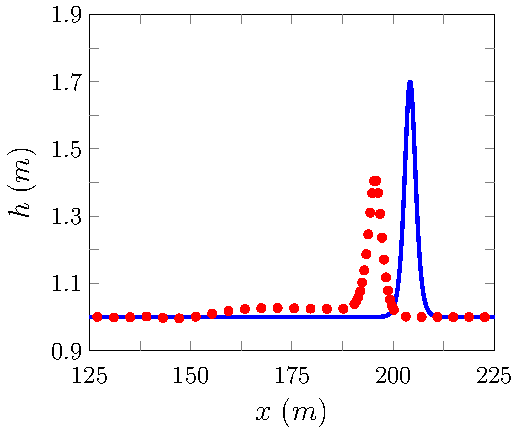
\includegraphics[width=\textwidth]{./chp5/figures/Analytic/Soliton/Example/FDVM1.pdf}
		\subcaption{$\text{FDVM}_1$}
		\vspace{0.5cm}
	\end{subfigure}%
	\begin{subfigure}{0.5\textwidth}
		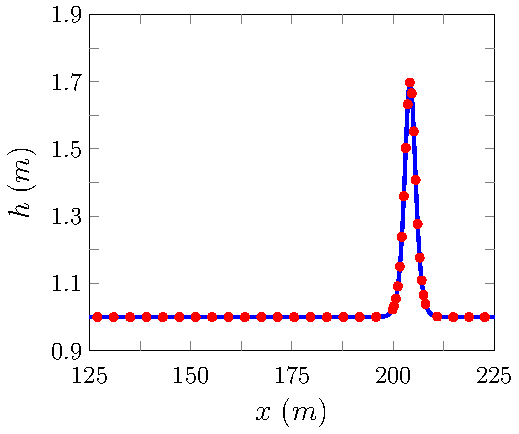
\includegraphics[width=\textwidth]{./chp5/figures/Analytic/Soliton/Example/FDVM2.pdf}
		\subcaption{$\text{FDVM}_2$}
		\vspace{0.5cm}
	\end{subfigure}
	\begin{subfigure}{0.5\textwidth}
		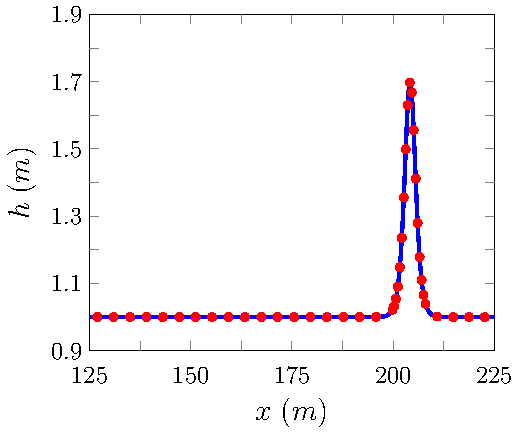
\includegraphics[width=\textwidth]{./chp5/figures/Analytic/Soliton/Example/FEVM2.pdf}
		\subcaption{$\text{FEVM}_2$}
		\vspace{0.5cm}
	\end{subfigure}%
	\begin{subfigure}{0.5\textwidth}
		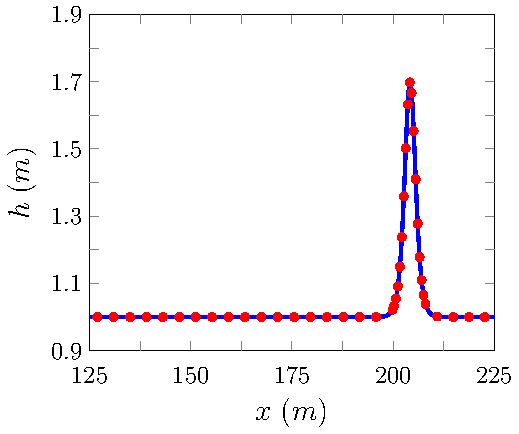
\includegraphics[width=\textwidth]{./chp5/figures/Analytic/Soliton/Example/FDVM3.pdf}
		\subcaption{$\text{FDVM}_3$}
		\vspace{0.5cm}
	\end{subfigure}
	\begin{subfigure}{0.5\textwidth}
		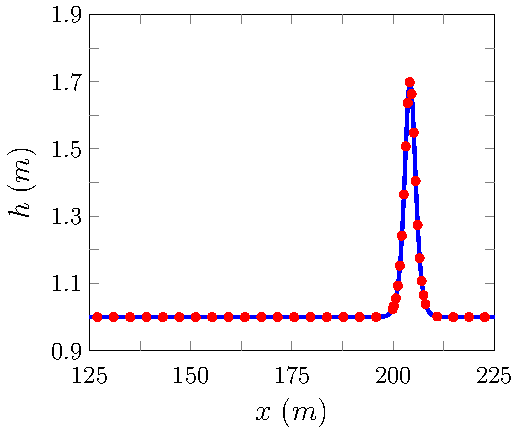
\includegraphics[width=\textwidth]{./chp5/figures/Analytic/Soliton/Example/D.pdf}
		\subcaption{$\mathcal{D}$}
	\end{subfigure}%
	\begin{subfigure}{0.5\textwidth}
		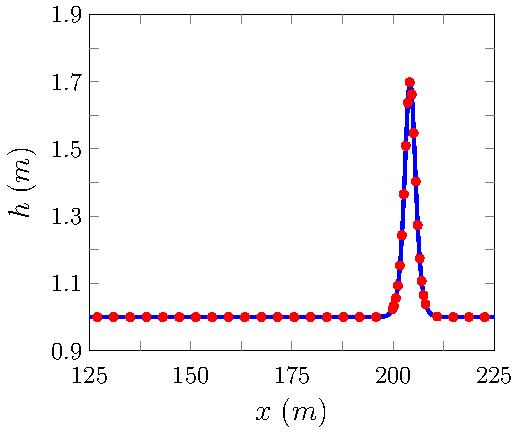
\includegraphics[width=\textwidth]{./chp5/figures/Analytic/Soliton/Example/W.pdf}
		\subcaption{$\mathcal{W}$}
	\end{subfigure}
	\caption{Comparison of the analytic solution ({\color{blue} \solidrule}) and numerical solution with $\Delta x = {100} / {2^{11}}m$ ({\color{red} $\bullet$}) for the soliton problem at $t=50s$ for all methods.}
	\label{fig:SolitonExAll}
\end{figure}


The $L_1$ norm was calculated for $h$, $u$ and $G$ for all numerical solutions and was plotted against $\Delta x$ for all numerical methods in Figure \ref{fig:SolitonL1All}. From these plots it is clear that all numerical methods are convergent. The rate at which the numerical solutions converge to the analytic solution over $\Delta x$ is determined by the order of accuracy of the numerical scheme. All methods demonstrate the expected order of accuracy given the order of accuracy of the approximations used in the method; which agrees with the results of the linear analysis in Chapter \ref{chp:AnalNumMethod}.  

\begin{figure}
	\centering
	\begin{subfigure}{0.5\textwidth}
		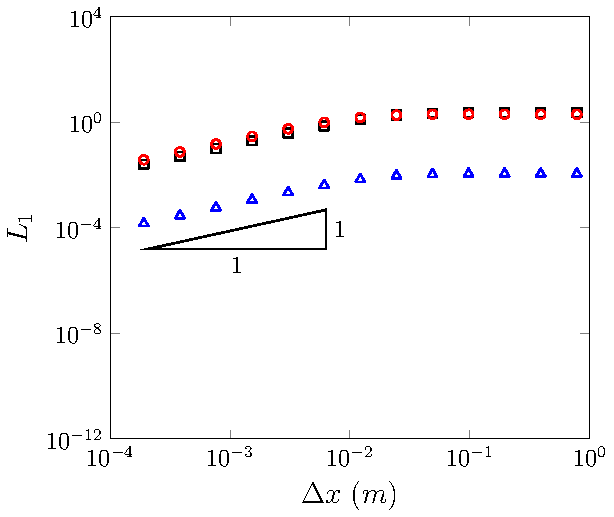
\includegraphics[width=\textwidth]{./chp5/figures/Analytic/Soliton/L1/FDVM1.pdf}
		\subcaption{$\text{FDVM}_1$}
		\vspace{0.5cm}
	\end{subfigure}%
	\begin{subfigure}{0.5\textwidth}
		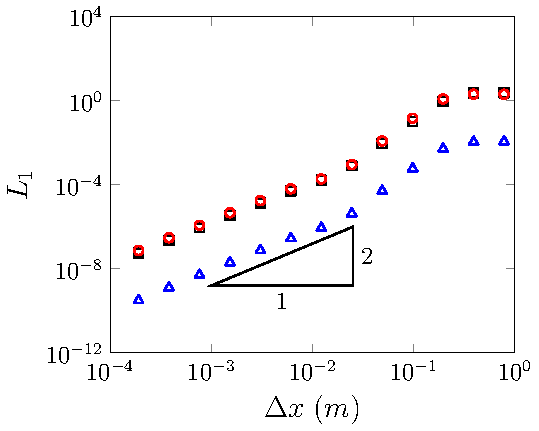
\includegraphics[width=\textwidth]{./chp5/figures/Analytic/Soliton/L1/FDVM2.pdf}
		\subcaption{$\text{FDVM}_2$}
		\vspace{0.5cm}
	\end{subfigure}
	\begin{subfigure}{0.5\textwidth}
		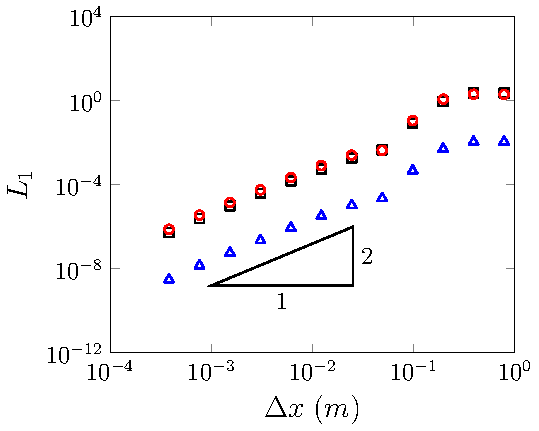
\includegraphics[width=\textwidth]{./chp5/figures/Analytic/Soliton/L1/FEVM2.pdf}
		\subcaption{$\text{FEVM}_2$}
		\vspace{0.5cm}
	\end{subfigure}%
	\begin{subfigure}{0.5\textwidth}
		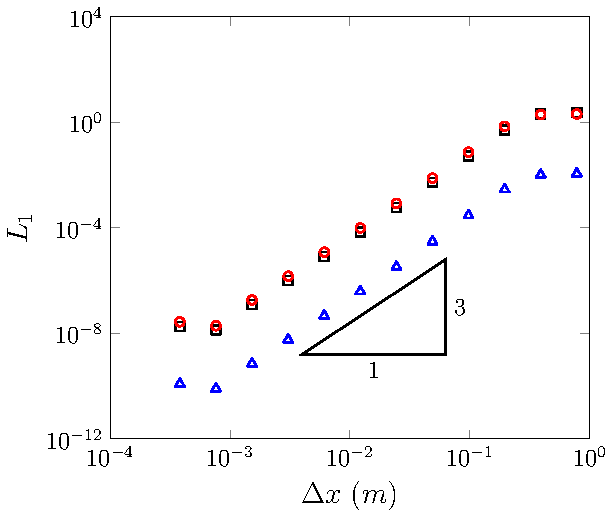
\includegraphics[width=\textwidth]{./chp5/figures/Analytic/Soliton/L1/FDVM3.pdf}
		\subcaption{$\text{FDVM}_3$}
		\vspace{0.5cm}
	\end{subfigure}
	\begin{subfigure}{0.5\textwidth}
		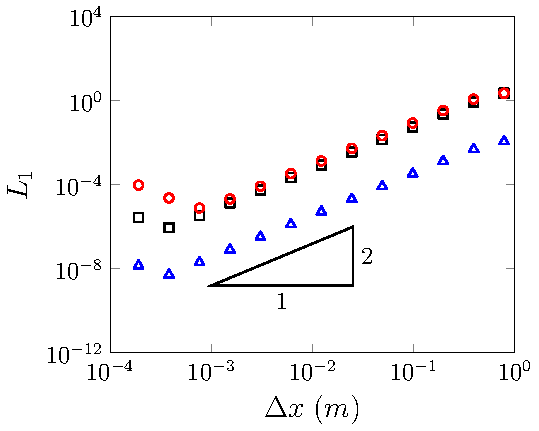
\includegraphics[width=\textwidth]{./chp5/figures/Analytic/Soliton/L1/D.pdf}
		\subcaption{$\mathcal{D}$}
	\end{subfigure}%
	\begin{subfigure}{0.5\textwidth}
		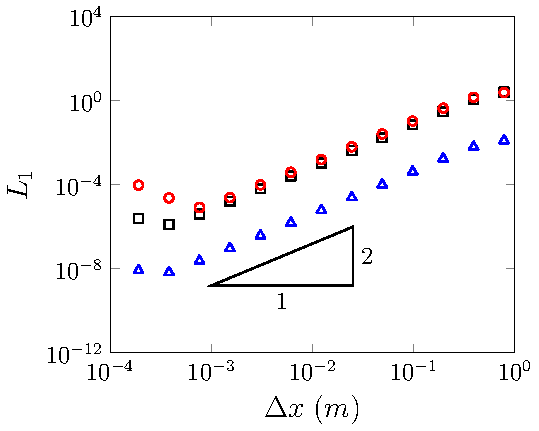
\includegraphics[width=\textwidth]{./chp5/figures/Analytic/Soliton/L1/W.pdf}
		\subcaption{$\mathcal{W}$}
	\end{subfigure}
	\caption{Convergence plots as measured by the $L_1$ norm for $h$ (\trianglet{blue}), $u$ (\squaret{black}) and $G$ (\circlet{red}) for the soliton problem for all methods.}
	\label{fig:SolitonL1All}
\end{figure}

All methods more accurately reproduced the analytic solution for $h$ than either $G$ or $u$ across all $\Delta x$ values. This is due to the simplicity of $h$'s evolution equation \eqref{eqn:FullSerreConMass} compared to the evolution equation of $G$ \eqref{eqn:Serreconsconmom}; with the error in $u$ being dominated by the error in $G$. 

Increasing the order of accuracy of our numerical methods leads to smaller errors when comparing two methods for the same $\Delta x$ value, as Figure \ref{fig:SolitonL1All} clearly demonstrates. This is consistent with the example numerical solution in Figure \ref{fig:SolitonExAll}, where the lowest order accuracy scheme, $\text{FDVM}_1$ had the poorest reproduction of the analytic solution. However, the benefit of increasing the order of accuracy is significantly diminished for the the third accurate $\text{FDVM}_3$ over the second-order $\text{FEVM}_2$ and $\text{FDVM}_2$.

For the second-order methods we find that $\text{FDVM}_2$ consistently produces the smallest $L_1$ error followed by $\text{FEVM}_2$, $\mathcal{W}$ and $\mathcal{D}$. The difference between the $\text{FDVM}_2$ and $\text{FEVM}_2$ is significant with errors of $\text{FEVM}_2$ being $2$ to $4$ times larger than $\text{FDVM}_2$. Therefore, $\text{FDVM}_2$ is reproducing the solitary wave solution more accurately than $\text{FEVM}_2$.

The finite difference methods produce very similar errors which are twice as large as the errors from $\text{FEVM}_2$. Additionally, the round-off effects which increase the $L_1$ error of the finite difference methods occur for larger $\Delta x$ values than the hybrid finite volume methods.

The error in conservation $C_1$ was calculated for all methods using the analytic expressions for the total amounts of the conserved quantities in the initial conditions \eqref{eqn:SolitonConservation}. The error in conservation was plotted against the spatial resolution in Figure \ref{fig:SolitonC1All}. These results demonstrate that due to the use of the finite volume methods for $h$ and $G$, both are conserved at round-off error for all the hybrid finite volume methods as expected. While the finite difference methods only conserved $h$ at round-off error because the employed finite difference method for the continuity equation \eqref{eqn:FullSerreConMass} is a conservative method. 

\begin{figure}
	\centering
	\begin{subfigure}{0.5\textwidth}
		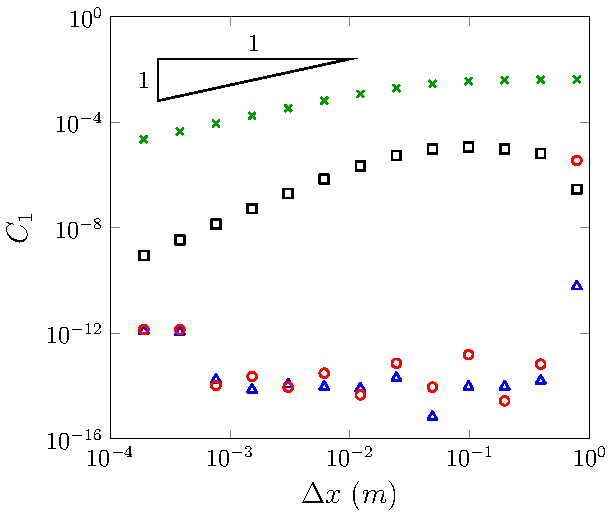
\includegraphics[width=\textwidth]{./chp5/figures/Analytic/Soliton/C1/FDVM1.pdf}
		\subcaption{$\text{FDVM}_1$}
		\vspace{0.3cm}
	\end{subfigure}%
	\begin{subfigure}{0.5\textwidth}
		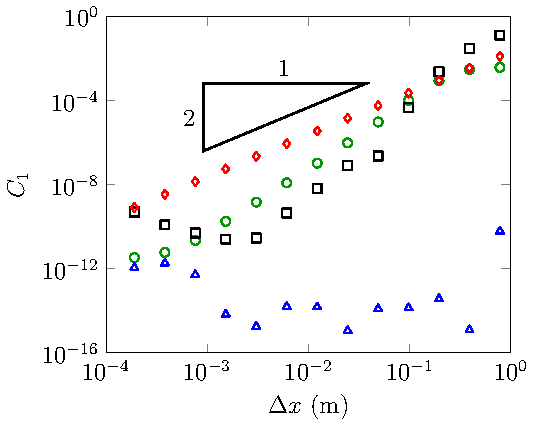
\includegraphics[width=\textwidth]{./chp5/figures/Analytic/Soliton/C1/FDVM2.pdf}
		\subcaption{$\text{FDVM}_2$}
		\vspace{0.3cm}
	\end{subfigure}
	\begin{subfigure}{0.5\textwidth}
		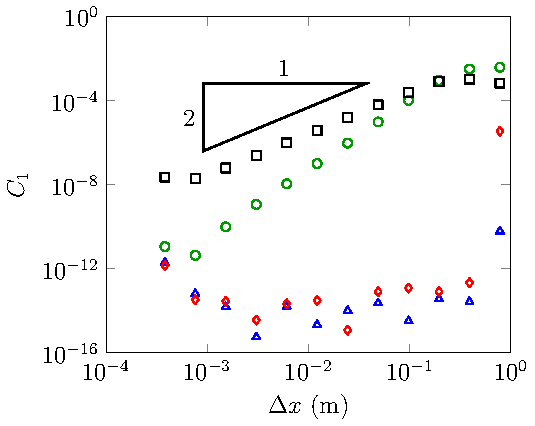
\includegraphics[width=\textwidth]{./chp5/figures/Analytic/Soliton/C1/FEVM2.pdf}
		\subcaption{$\text{FEVM}_2$}
		\vspace{0.3cm}
	\end{subfigure}%
	\begin{subfigure}{0.5\textwidth}
		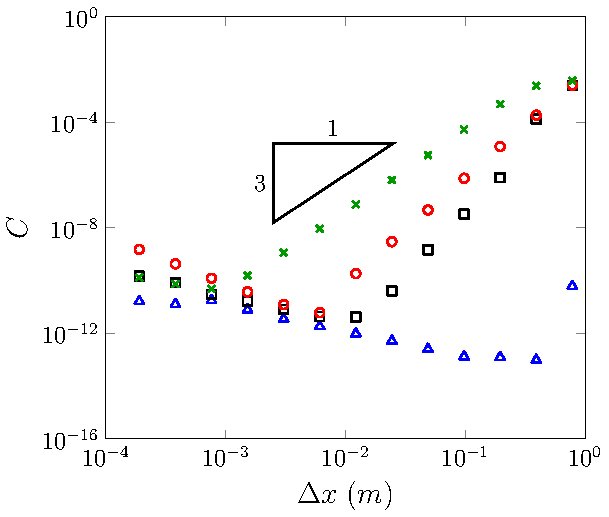
\includegraphics[width=\textwidth]{./chp5/figures/Analytic/Soliton/C1/FDVM3.pdf}
		\subcaption{$\text{FDVM}_3$}
		\vspace{0.3cm}
	\end{subfigure}
	\begin{subfigure}{0.5\textwidth}
		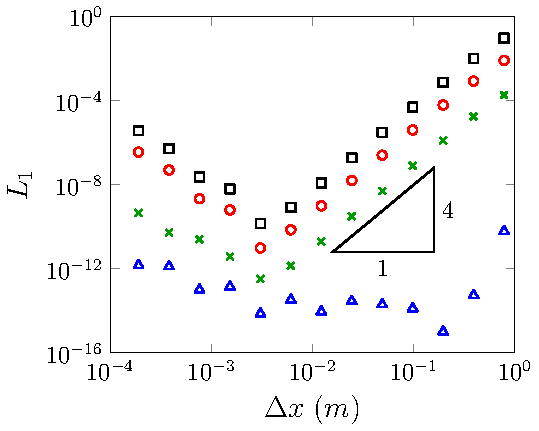
\includegraphics[width=\textwidth]{./chp5/figures/Analytic/Soliton/C1/D.pdf}
		\subcaption{$\mathcal{D}$}
	\end{subfigure}%
	\begin{subfigure}{0.5\textwidth}
		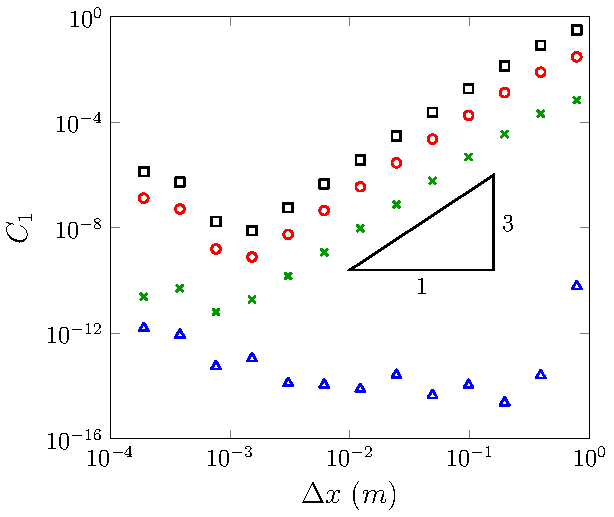
\includegraphics[width=\textwidth]{./chp5/figures/Analytic/Soliton/C1/W.pdf}
		\subcaption{$\mathcal{W}$}
	\end{subfigure}
	\caption{Conservation plots as measured by $C_1$ for $h$ (\trianglet{blue}), $uh$ (\squaret{black}), $G$ (\circlet{red}) and $\mathcal{H}$ ({\crosst{green!60!black}}) for the soliton problem for all methods.}
	\label{fig:SolitonC1All}
\end{figure}

No methods conserve the energy $\mathcal{H}$ or the momentum $uh$ at machine precision. Since none of the methods were designed to have these as conserved variables this is not surprising, although the error in conservation of all methods for these quantities does inherit the order of accuracy of the convergence of the numerical method or better, as expected. 

For small $\Delta x$ values the round-off errors become dominant, particularly for the finite difference methods. Interestingly, $\text{FDVM}_3$ has an accumulation of round-off error in the conservation error for $h$ and $G$ as $\Delta x$ decreases. This was found to be caused by the Runge-Kutta coefficients \cite{Zoppou-etal-2017} which in the last step are $1/3$ and $2/3$ which cannot be exactly represented in floating point, so that every time step accumulates a small conservation errors of machine precision size leading to the observed increase as $\Delta x$ becomes small and the number of time steps increases.

These results demonstrate the need for higher-order accurate schemes to accurately approximate the Serre equations. Furthermore, they suggest that second-order accuracy is sufficient, with third-order accurate schemes showing only a slight improvement. Finally they also demonstrate the utility of these hybrid FVM for conserving $h$ and $G$, as desired. Given these results, only $\text{FEVM}_2$ and $\text{FDVM}_2$ have been extended to allow for variable bathymetry and dry beds. Consequently, the rest of the results in this chapter and Chapter \ref{chp:ExpMethodComp} will only be for these numerical methods. 



\section{Analytic Solution for Variable Bathymetry}
To verify the validity of our numerical methods for the Serre equations with variable bathymetry and assess the well balancing method we compare various numerical solutions to the lake at rest analytic stationary solution given by \eqref{eqn:LARdefhub}. 

The particular lake at rest solution \eqref{eqn:LARdefhub} associated with the bed profile
\begin{equation}
b(x) = a_1 \sin\left(a_2 x\right)
\end{equation}
was chosen for this validation to ensure that all terms with derivatives of the bed were tested. To demonstrate the capability of the methods in the presence of dry and wet beds the parameter values $a_0 = 0m$, $a_1 = 1m$ and $a_2 = 2 \pi / 50 m^{-1} $ were chosen. These parameter values result in a periodic bed where water with a constant stage submerges the troughs of the bed while the peaks of the bed are dry. 

For the numerical solutions the spatial domain was $x \in \left[-112.5 m,87.5 m\right]$ and the final time was $t=10s$, with the standard gravitational acceleration $g= 9.81 m/s^2$. The spatial resolution of the method was varied so that $\Delta x = 100 / 2^k m$ with $k \in \left[8, \dots  ,17\right]$ and the CFL condition \eqref{eqn:CFLcond} was satisfied by having $\Delta t = Cr \Delta x / \sqrt{g}$ with condition number $Cr = 0.5$. The standard limiting parameter $\theta = 1.2$ was used in the generalised minmod limiter, \eqref{eqn:slopehGrecon} for both $\text{FEVM}_2$ and $\text{FDVM}_2$. Dirichlet boundary conditions were used at both ends as the analytic solution is stationary.

The numerical methods are assessed by using the specified lake at rest solution as initial conditions and comparing the numerical solutions of $\text{FEVM}_2$ and $\text{FDVM}_2$ at $t=10s$ to the analytic solution, which are the initial conditions. To demonstrate the utility of the well balancing method the results from two versions of $\text{FEVM}_2$ and $\text{FDVM}_2$ are presented, where the well balancing method described in Chapter \ref{chp:HFVMMethod} is and isn't employed.   

\subsection{Results for Lake at Rest}
Example numerical solutions with $\Delta x = 100/2^{10}m \approx 0.0977m$ at $t=10s$ for all versions of $\text{FEVM}_2$ and $\text{FDVM}_2$ are given in Figure \ref{fig:LakeAtRestEx}. The numerical solutions in these figures are indistinguishable from the analytic solutions at this scale and so the analytic solutions have been omitted from the plots.  

\begin{figure}
	\centering
	\begin{subfigure}{0.5\textwidth}
		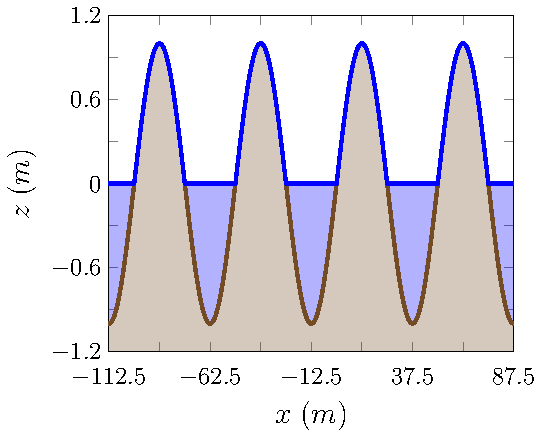
\includegraphics[width=\textwidth]{./chp5/figures/Analytic/LakeAtRest/Example/FEVMWB.pdf}
		\subcaption{$\text{FEVM}_2$ well balanced}
		\vspace{0.5cm}
	\end{subfigure}%
	\begin{subfigure}{0.5\textwidth}
		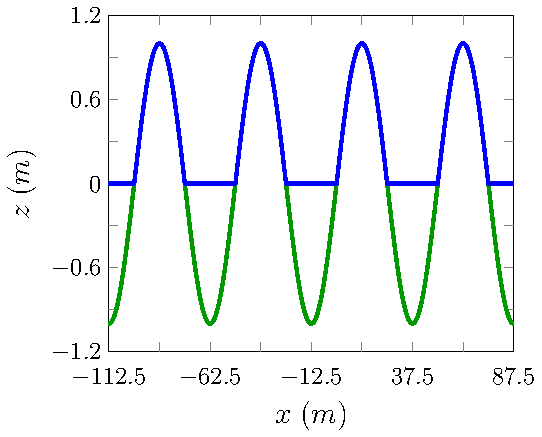
\includegraphics[width=\textwidth]{./chp5/figures/Analytic/LakeAtRest/Example/FEVMnWB.pdf}
		\subcaption{$\text{FEVM}_2$ not well balanced}
		\vspace{0.5cm}
	\end{subfigure}
	\begin{subfigure}{0.5\textwidth}
		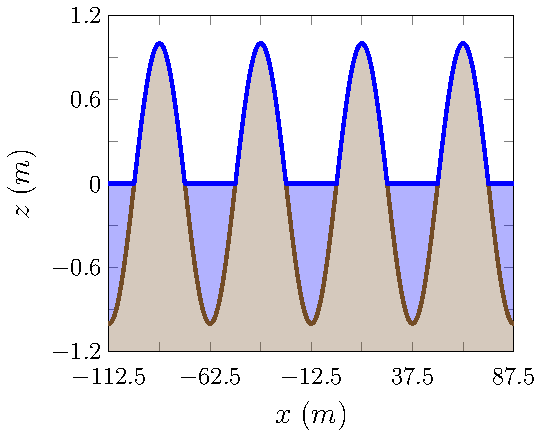
\includegraphics[width=\textwidth]{./chp5/figures/Analytic/LakeAtRest/Example/FDVMWB.pdf}
		\subcaption{$\text{FDVM}_2$ well balanced}
	\end{subfigure}%
	\begin{subfigure}{0.5\textwidth}
		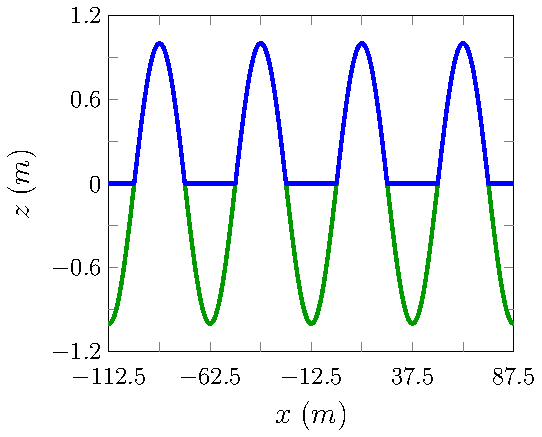
\includegraphics[width=\textwidth]{./chp5/figures/Analytic/LakeAtRest/Example/FDVMnWB.pdf}
		\subcaption{$\text{FDVM}_2$ not well balanced}
	\end{subfigure}
	\caption{Plot of numerical solutions for $w$ (\squareF{blue}) and $b$ (\squareF{brown!60!black}) with $\Delta x = {100} / {2^{10}}m $ for the lake at rest problem at $t=10s$ for all methods.}
	\label{fig:LakeAtRestEx}
\end{figure}

%[]Expalin second order of slopes increase?
Examination of the $L_1$ errors depicted in Figure \ref{fig:LakeAtRestEL1} reveals that only  the well balanced methods have accurately recovered the analytic solution. With both well balanced versions of the methods reproducing $h$, $G$ and $u$ precisely, accounting for round-off errors. This is most clear for $h$ as it is consistently around the machine epsilon value. While for $G$ and $u$ their error is increasing due to an accumulation of the round-off errors for each cell and time step; hence their second-order increase as $\Delta x \rightarrow 0$.

\begin{figure}
	\centering
	\begin{subfigure}{0.5\textwidth}
		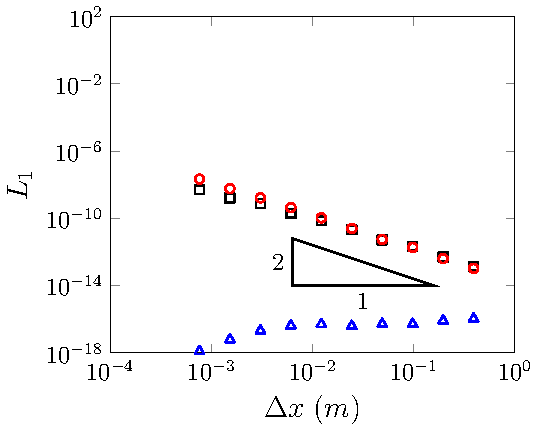
\includegraphics[width=\textwidth]{./chp5/figures/Analytic/LakeAtRest/L1/FEVMWB.pdf}
		\subcaption{$\text{FEVM}_2$ well balanced}
		\vspace{0.3cm}
	\end{subfigure}%
	\begin{subfigure}{0.5\textwidth}
		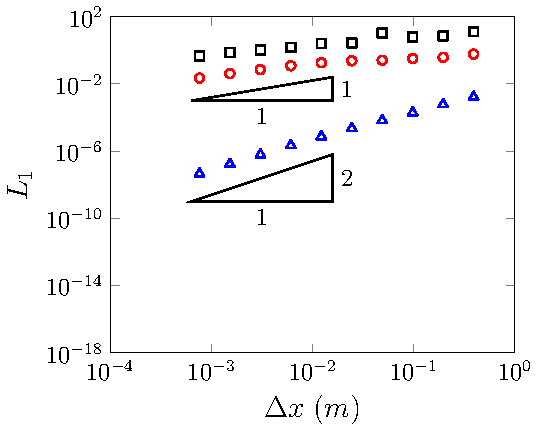
\includegraphics[width=\textwidth]{./chp5/figures/Analytic/LakeAtRest/L1/FEVMnWB.pdf}
		\subcaption{$\text{FEVM}_2$ not well balanced}
		\vspace{0.3cm}
	\end{subfigure}
	\begin{subfigure}{0.5\textwidth}
		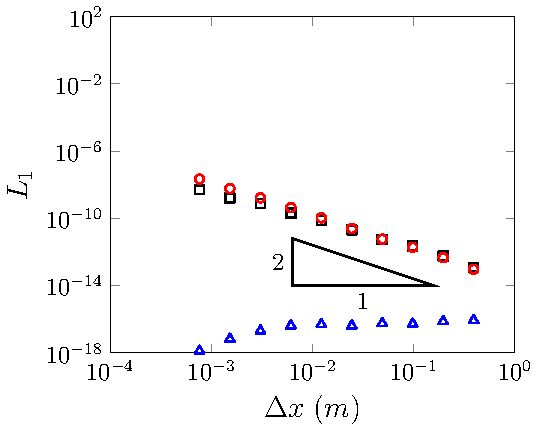
\includegraphics[width=\textwidth]{./chp5/figures/Analytic/LakeAtRest/L1/FDVMWB.pdf}
		\subcaption{$\text{FDVM}_2$ well balanced}
	\end{subfigure}%
	\begin{subfigure}{0.5\textwidth}
		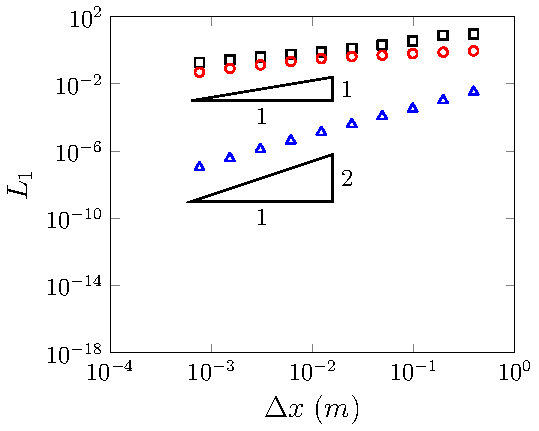
\includegraphics[width=\textwidth]{./chp5/figures/Analytic/LakeAtRest/L1/FDVMnWB.pdf}
		\subcaption{$\text{FDVM}_2$ not well balanced}
	\end{subfigure}
	\caption{Convergence plots as measured by the $L_1$ norm for $h$ (\trianglet{blue}), $u$ (\squaret{black}) and $G$ (\circlet{red}) for the lake at rest problem at $t=10s$ for all methods.}
	\label{fig:LakeAtRestEL1}
\end{figure}

For methods without well balancing; the errors are significantly larger, yet they are converging to the analytic solution. However, the convergence of these methods has lost an order of accuracy in $u$ and $G$; with only first-order convergence in these quantities and not the expected second-order accuracy observed for $h$. 

Using the expressions in Appendix \ref{app:ConQuant} for the total amounts of the conserved variables $C_1$ was calculated for all numerical solutions with the results plotted in Figure \ref{fig:LakeAtRestEC1}. The error in conservation of these methods affirms the superiority of the well-balanced version of the methods. For the well balanced $\text{FEVM}_2$ the conservation of $h$ and $\mathcal{H}$ has zero error and so could not be represented on the log-log plot, so that all errors in conservation are at machine precision or lower. For the well-balanced $\text{FDVM}_2$ the error in $h$ vanishes when $\Delta x$ is small, although the error in $\mathcal{H}$ does not. Therefore, the well balanced version of $\text{FEVM}_2$ outperforms the $\text{FDVM}_2$ in this instance. While for the methods with no well balancing none of the quantities are conserved at machine precision. 

\begin{figure}
	\centering
	\begin{subfigure}{0.5\textwidth}
		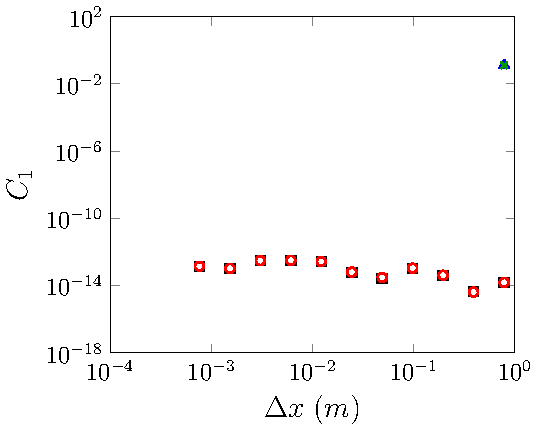
\includegraphics[width=\textwidth]{./chp5/figures/Analytic/LakeAtRest/C1/FEVMWB.pdf}
		\subcaption{$\text{FEVM}_2$ well balanced}
		\vspace{0.5cm}
	\end{subfigure}%
	\begin{subfigure}{0.5\textwidth}
		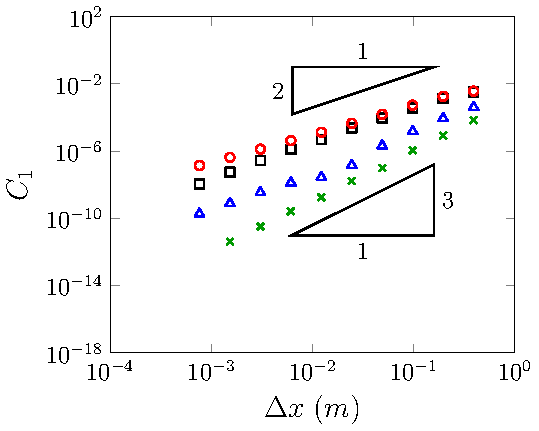
\includegraphics[width=\textwidth]{./chp5/figures/Analytic/LakeAtRest/C1/FEVMnWB.pdf}
		\subcaption{$\text{FEVM}_2$ not well balanced}
		\vspace{0.5cm}
	\end{subfigure}
	\begin{subfigure}{0.5\textwidth}
		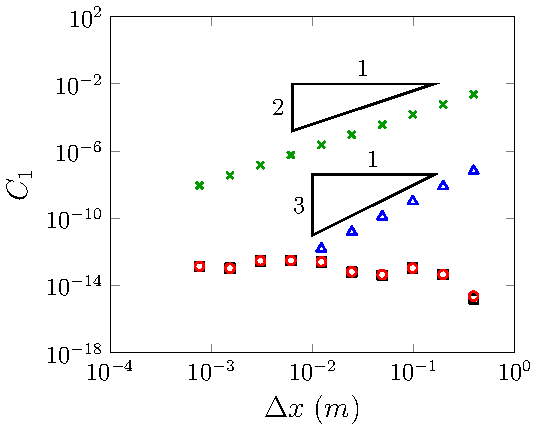
\includegraphics[width=\textwidth]{./chp5/figures/Analytic/LakeAtRest/C1/FDVMWB.pdf}
		\subcaption{$\text{FDVM}_2$ well balanced}
	\end{subfigure}%
	\begin{subfigure}{0.5\textwidth}
		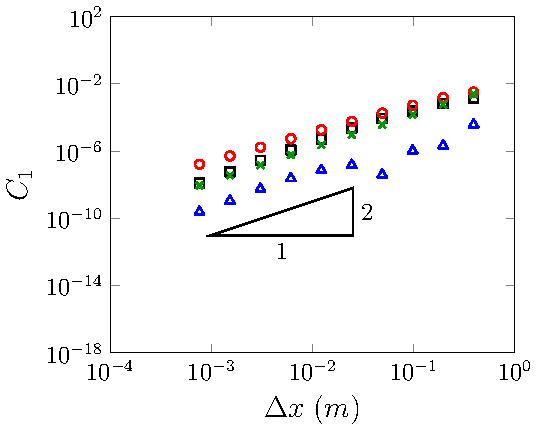
\includegraphics[width=\textwidth]{./chp5/figures/Analytic/LakeAtRest/C1/FDVMnWB.pdf}
		\subcaption{$\text{FDVM}_2$ not well balanced}
	\end{subfigure}
	\caption{$C_1$ error against $\Delta x$ for $h$ (\trianglet{blue}), $uh$ (\squaret{black}), $G$ (\circlet{red}) and $\mathcal{H}$ ({\color{green!60!black} \crosst{green!60!black}}) for the lake at rest problem at $t=10s$ for all methods.}
	\label{fig:LakeAtRestEC1}
\end{figure}  

These results demonstrate the need for the well-balancing for both numerical methods, as it is only with their inclusion that the lake at rest steady state can be accurately reproduced. 


\section{Forced Solutions}
%only L1
There are currently no known analytic solutions for the Serre equations that possess varying bathymetry and non-zero velocities. Therefore, the previous analytic solution validations do not provide a stringent test for all terms present in the Serre equations. To remedy this the forced solutions introduced in Chapter \ref{chp:Serreeqns} were used. Since the source terms in the modified Serre equations, \eqref{eqn:FullSerreConForced} can be determined and accounted for analytically, the only source of error in the numerical solutions reproduction of the forced solutions are the numerical methods themselves and thus the theoretical second-order accuracy of $\text{FEVM}_2$ and $\text{FDVM}_2$ should be recovered. 

We performed validation tests for two forced solutions; one with a finite water depth everywhere and the other with a dry bed to validate and compare the numerical solutions in both situations. To ensure that all terms of the Serre equations were accurately approximated in the numerical method the functions
\begin{subequations}
\begin{align}
\label{eqn:ForcedSolutionxt}
h^*(x,t) &= a_0 + a_1 \exp\left(-\dfrac{\left[\left(x - a_2 t\right) - a_3\right]^2}{2 a_4}\right), \\
u^*(x,t) &= a_5 \exp\left(-\dfrac{\left[\left(x - a_2 t\right) - a_3\right]^2}{2 a_4}\right), \\
b^*(x) &= a_6 \sin\left(a_7 x\right)
\end{align}
\end{subequations}
for the primitive variables were chosen. These functions produce an $a_1$ high Gaussian bump for $h$ and $u$ that travels at a fixed speed $a_2$ over a periodic bed. For nontrivial choices of the parameters $a_i$ all terms in the Serre equations vary in space and time and so all terms must be accurately approximated by the numerical method to adequately reproduce the forced solution. 

Both validation studies used $a_1 = 0.5m$, $a_2 = 2 \pi / \left(10 a_7\right) m/s$, $a_3 = - 3\pi/ \left(2 a_7\right) m$, $a_4 = \pi / (16 a_7) m$, $a_5 = 0.5 m/s$, $a_6 = 1.0 m$ and $a_7 = \pi / 25 m^{-1}$ with $a_0= 1m$ for the finite water depth forced solution and $a_0=0m$ for the dry bed forced solution. These parameter values results in a Gaussian bump that has a width much smaller than the wavelength of the bed profile and travels precisely one wavelength in $10s$.

The domain of the numerical solutions was $x \in \left[-112.5 m,87.5 m\right]$ with $t \in \left[0s,10s\right]$. The standard gravitational acceleration $g= 9.81 m/s^2$ was used. The spatial resolution of numerical methods was varied like so $\Delta x = 100 / 2^k m$ with $k \in \left[8,\dots,16\right]$. To satisfy the CFL condition, \eqref{eqn:CFLcond} the temporal resolution
$\Delta t = Cr \Delta x / \left(a_2 + a_5 + \sqrt{g\left(a_0 + a_1\right)}\right)$ was chosen with condition number $Cr = 0.5$. The value $\theta = 1.2$ was used in the generalised minmod limiter \eqref{eqn:slopehGrecon} for both $\text{FEVM}_2$ and $\text{FDVM}_2$ and Dirichlet boundary conditions were applied at the boundaries of the domain. 


\subsection{Results for Finite Water Depth} 
%a_0 = 1
For the finite water depth case where $a_0 = 1m$ an example of the numerical solutions of $\text{FEVM}_2$ and $\text{FDVM}_2$ are given in Figures \ref{fig:ForcedWetFEVMP2PExAll} and \ref{fig:ForcedWetFDVMP2PExAll} respectively for $\Delta x = 100/ 2^{10} m \approx 0.0977m $ at various times. The numerical solutions and the forced solutions are identical at all times for these scales, accurately reproducing the forced solution as it travels over the bed.
\begin{figure}
	\centering
	\begin{subfigure}{0.5\textwidth}
		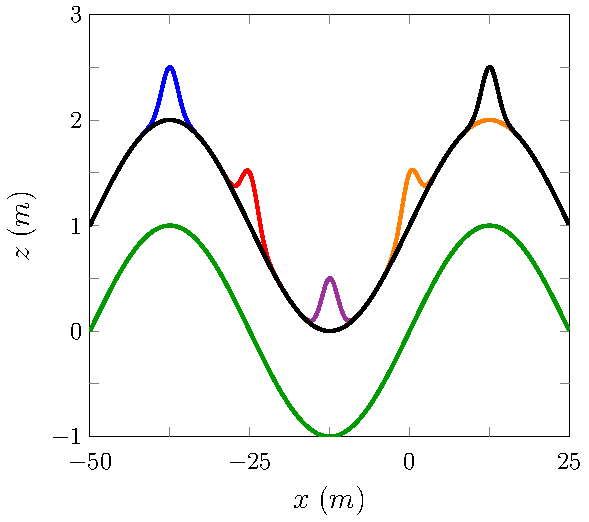
\includegraphics[width=\textwidth]{./chp5/figures/Forced/Wet/FEVMw.pdf}
		\subcaption{$w$ and $b$ (\squareF{brown!60!black})}
		\vspace{0.5cm}
	\end{subfigure}%
	\begin{subfigure}{0.5\textwidth}
		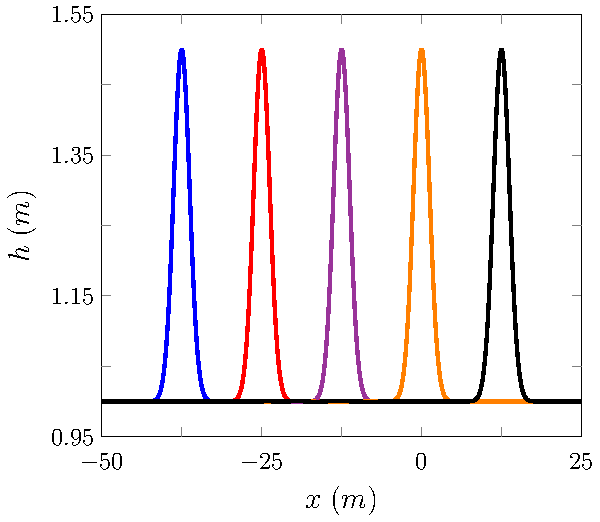
\includegraphics[width=\textwidth]{./chp5/figures/Forced/Wet/FEVMh.pdf}
		\subcaption{$h$}
		\vspace{0.5cm}
	\end{subfigure}
	\begin{subfigure}{0.5\textwidth}
		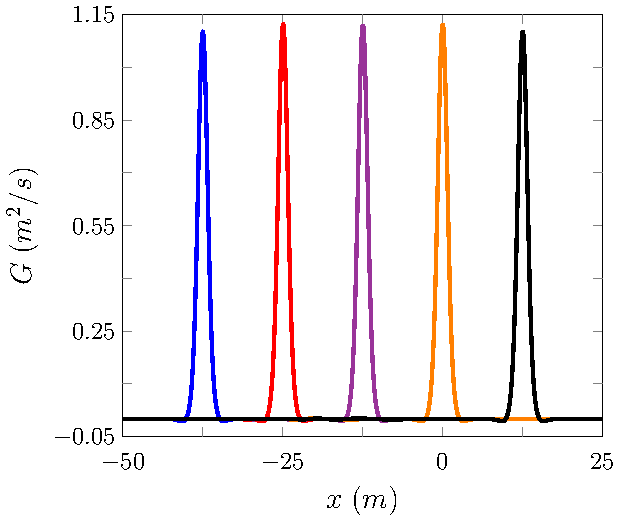
\includegraphics[width=\textwidth]{./chp5/figures/Forced/Wet/FEVMG.pdf}
		\subcaption{$G$}
	\end{subfigure}%
	\begin{subfigure}{0.5\textwidth}
		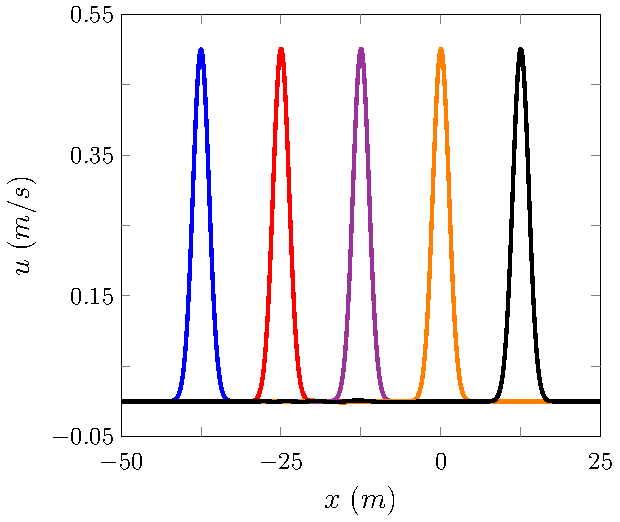
\includegraphics[width=\textwidth]{./chp5/figures/Forced/Wet/FEVMu.pdf}
		\subcaption{$u$}
	\end{subfigure}
	\caption{Plots of $w$, $b$, $h$, $G$ and $u$ produced by $\text{FEVM}_2$ with $\Delta x = 100 / 2^{10}m$ at $t=$ $0s$ ({\color{blue} \solidrule} / \squareF{blue} ), $2.5s$ ({\color{red} \solidrule}/ \squareF{red}), $5.0s$ ({\color{violet!80!white} \solidrule} / \squareF{violet!80!white}), $7.5s$ ({\color{orange} \solidrule}/ \squareF{orange}), $10.0s$ ({\color{black} \solidrule} / \squareF{black}) of the finite water depth forced solution problem, where $a_0 = 1m$.}
	\label{fig:ForcedWetFEVMP2PExAll}
\end{figure}
\begin{figure}
	\centering
	\begin{subfigure}{0.5\textwidth}
		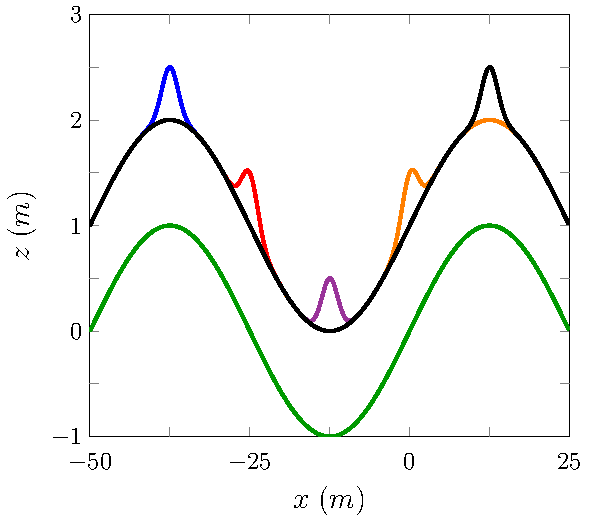
\includegraphics[width=\textwidth]{./chp5/figures/Forced/Wet/FDVMw.pdf}
		\subcaption{$w$ and $b$ (\squareF{brown!60!black})}
		\vspace{0.5cm}
	\end{subfigure}%
	\begin{subfigure}{0.5\textwidth}
		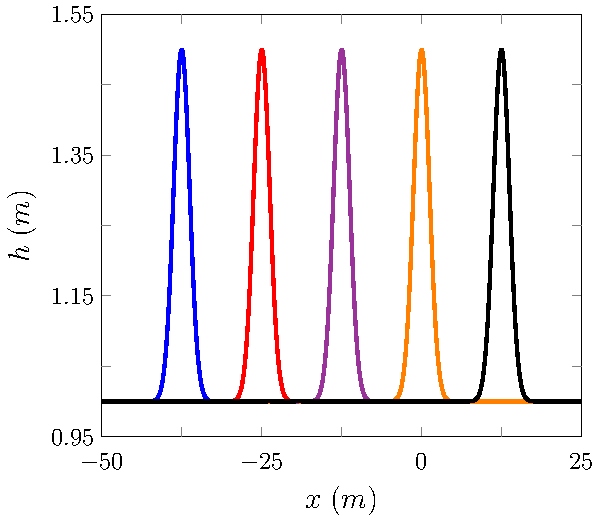
\includegraphics[width=\textwidth]{./chp5/figures/Forced/Wet/FDVMh.pdf}
		\subcaption{$h$}
		\vspace{0.5cm}
	\end{subfigure}
	\begin{subfigure}{0.5\textwidth}
		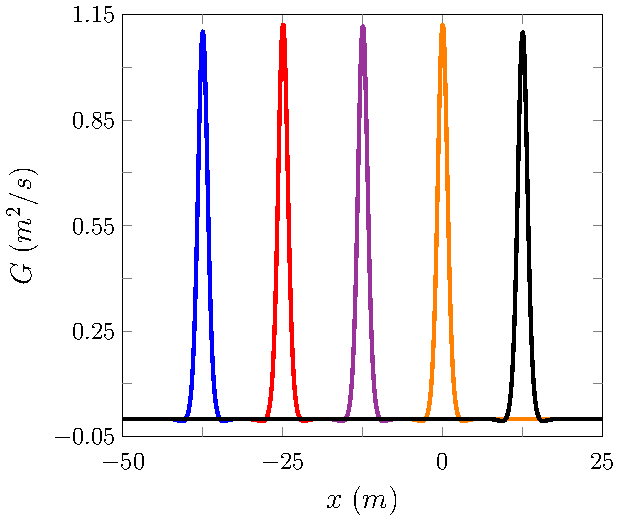
\includegraphics[width=\textwidth]{./chp5/figures/Forced/Wet/FDVMG.pdf}
		\subcaption{$G$}
	\end{subfigure}%
	\begin{subfigure}{0.5\textwidth}
		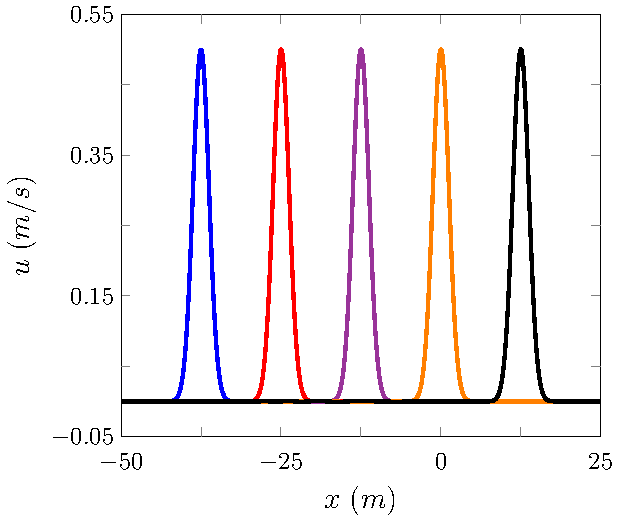
\includegraphics[width=\textwidth]{./chp5/figures/Forced/Wet/FDVMu.pdf}
		\subcaption{$u$}
	\end{subfigure}
	\caption{Plots of $w$, $b$, $h$, $G$ and $u$ produced by $\text{FDVM}_2$ with $\Delta x = 100 / 2^{10}m$ at $t=$ $0s$ ({\color{blue} \solidrule} / \squareF{blue} ), $2.5s$ ({\color{red} \solidrule}/ \squareF{red}), $5.0s$ ({\color{violet!80!white} \solidrule} / \squareF{violet!80!white}), $7.5s$ ({\color{orange} \solidrule}/ \squareF{orange}), $10.0s$ ({\color{black} \solidrule} / \squareF{black}) of the finite water depth forced solution problem, where $a_0 = 1m$.}
	\label{fig:ForcedWetFDVMP2PExAll}
\end{figure}

The $L_1$ error of $h$, $u$ and $G$ for the $\text{FEVM}_2$ and $\text{FDVM}_2$ are given in Figure \ref{fig:L1convergenceforcedWet}. Both methods recover the expected second-order accuracy. Since the source term of the modified Serre equations is added analytically and all terms must be accurately approximated by the method for this forced solution, these results demonstrate that our scheme is second-order accurate for all terms when the bed is wet everywhere, as desired.

\begin{figure}
	\centering
	\begin{subfigure}{0.5\textwidth}
		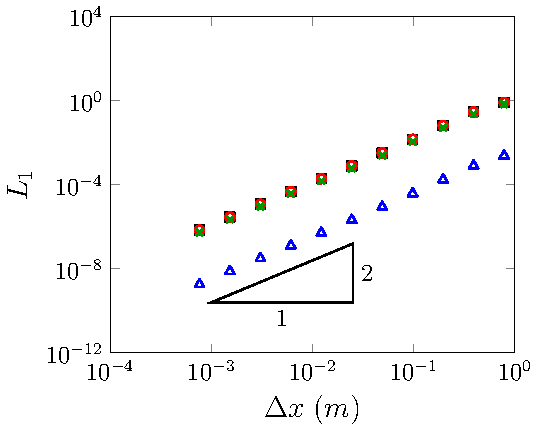
\includegraphics[width=\textwidth]{./chp5/figures/Forced/Wet/FEVML1.pdf}
		\subcaption{$\text{FEVM}_2$}
	\end{subfigure}%
	%[]!!---!![]
	\begin{subfigure}{0.5\textwidth}
		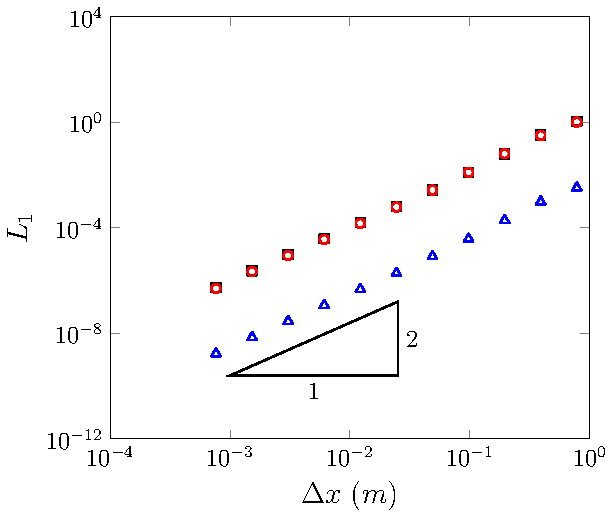
\includegraphics[width=\textwidth]{./chp5/figures/Forced/Wet/FDVML1.pdf}
		\subcaption{$\text{FDVM}_2$}
	\end{subfigure}
	\caption{Convergence plots as measured by the $L_1$ norm for $h$ (\trianglet{blue}), $u$ (\squaret{black}) and $G$ (\circlet{red}) for the finite water forced solution problem for FEVM and FDVM at $t=10s$.}
	\label{fig:L1convergenceforcedWet}
\end{figure}


\subsection{Results with Dry Beds} 
%a_0 = 0
%mention the tolerance values
To demonstrate the capability of the methods to handle wetting and drying of beds, a series of numerical simulations of the forced solutions \eqref{eqn:ForcedSolutionxt} where $a_0 = 0m$ were conducted using both $\text{FEVM}_2$ and $\text{FDVM}_2$. 

Example numerical solutions demonstrating the evolution of the wave are given in Figure \ref{fig:ForcedFEVMP2PExAll} for $\text{FEVM}_2$ and Figure \ref{fig:ForcedFDVMP2PExAll} $\text{FDVM}_2$ with $\Delta x = 100/ 2^{10} m \approx 0.0977m$ at various times. The methods accurately reproduce the analytic solution for the stage $w$, $h$ and $G$. However, both fail to accurately reproduce $u$ when $h$ is small, particularly behind the wave.

\begin{figure}
	\centering
	\begin{subfigure}{0.5\textwidth}
		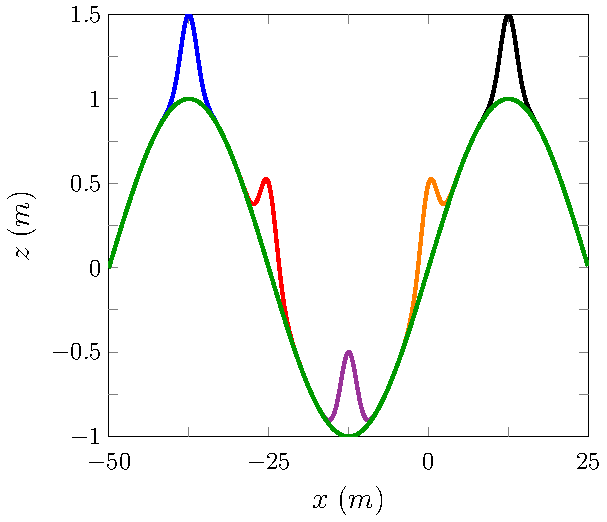
\includegraphics[width=\textwidth]{./chp5/figures/Forced/Dry/FEVMw.pdf}
		\subcaption{$w$ and $b$ (\squareF{brown!60!black})}
		\vspace{0.5cm}
	\end{subfigure}%
	\begin{subfigure}{0.5\textwidth}
		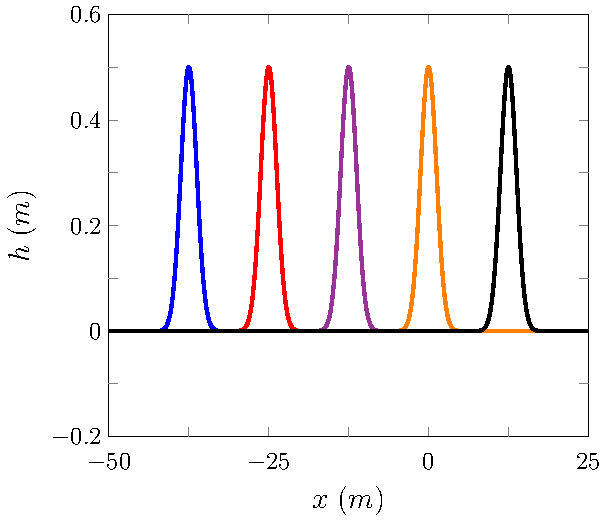
\includegraphics[width=\textwidth]{./chp5/figures/Forced/Dry/FEVMh.pdf}
		\subcaption{$h$}
		\vspace{0.5cm}
	\end{subfigure}
	\begin{subfigure}{0.5\textwidth}
		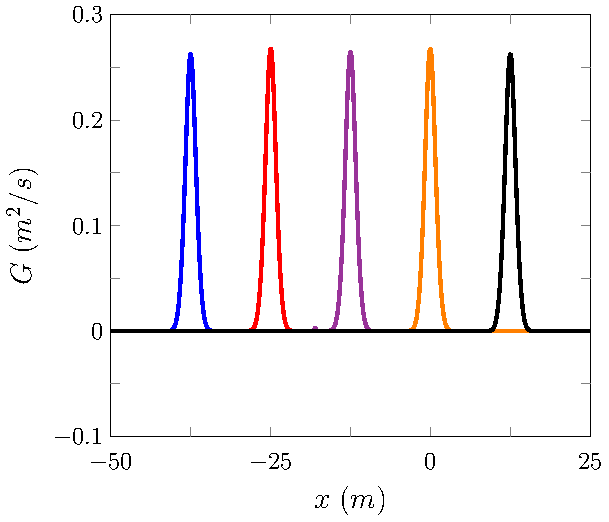
\includegraphics[width=\textwidth]{./chp5/figures/Forced/Dry/FEVMG.pdf}
		\subcaption{$G$}
	\end{subfigure}%
	\begin{subfigure}{0.5\textwidth}
		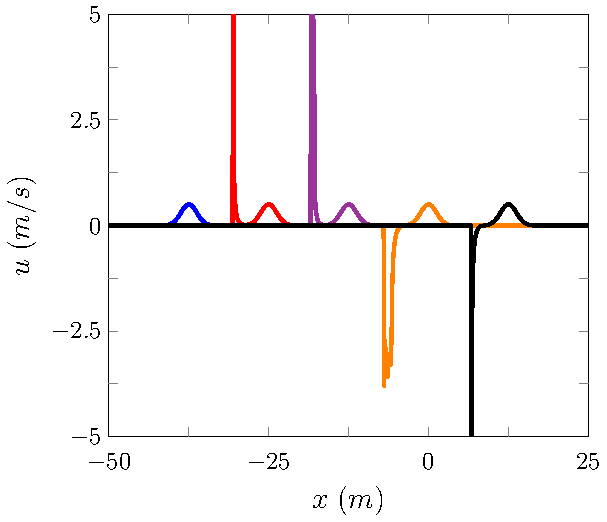
\includegraphics[width=\textwidth]{./chp5/figures/Forced/Dry/FEVMu.pdf}
		\subcaption{$u$}
	\end{subfigure}
	\caption{Plots of $w$, $b$, $h$, $G$ and $u$ produced by $\text{FEVM}_2$ with $\Delta x = 100 / 2^{10}m$ at $t=$ $0s$ ({\color{blue} \solidrule} / \squareF{blue} ), $2.5s$ ({\color{red} \solidrule}/ \squareF{red}), $5.0s$ ({\color{violet!80!white} \solidrule} / \squareF{violet!80!white}), $7.5s$ ({\color{orange} \solidrule}/ \squareF{orange}), $10.0s$ ({\color{black} \solidrule} / \squareF{black}) of the dry bed forced solution problem, where $a_0 = 0m$.}
	\label{fig:ForcedFEVMP2PExAll}
\end{figure}
\begin{figure}
	\centering
	\begin{subfigure}{0.5\textwidth}
		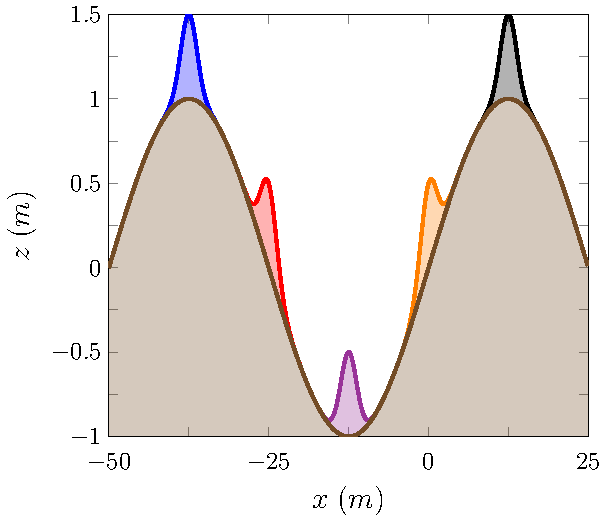
\includegraphics[width=\textwidth]{./chp5/figures/Forced/Dry/FDVMw.pdf}
		\subcaption{$w$ and $b$ (\squareF{brown!60!black})}
		\vspace{0.5cm}
	\end{subfigure}%
	\begin{subfigure}{0.5\textwidth}
		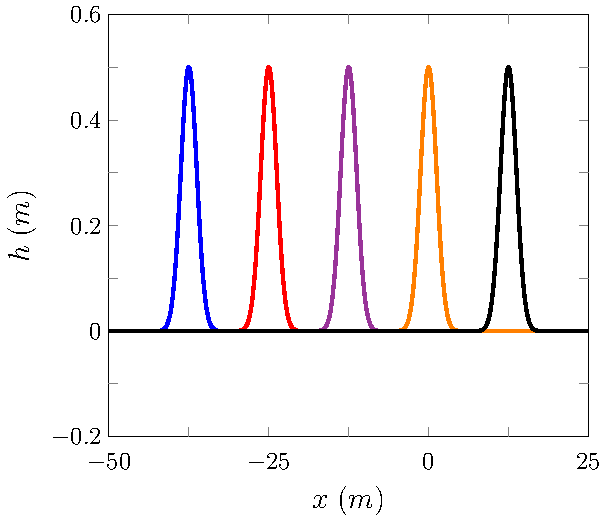
\includegraphics[width=\textwidth]{./chp5/figures/Forced/Dry/FDVMh.pdf}
		\subcaption{$h$}
		\vspace{0.5cm}
	\end{subfigure}
	\begin{subfigure}{0.5\textwidth}
		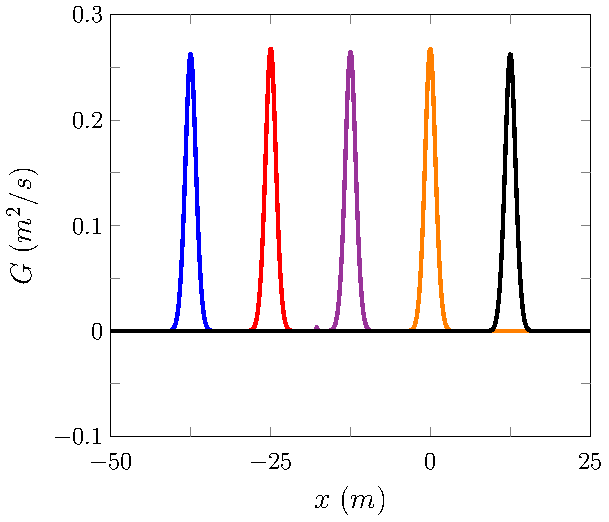
\includegraphics[width=\textwidth]{./chp5/figures/Forced/Dry/FDVMG.pdf}
		\subcaption{$G$}
	\end{subfigure}%
	\begin{subfigure}{0.5\textwidth}
		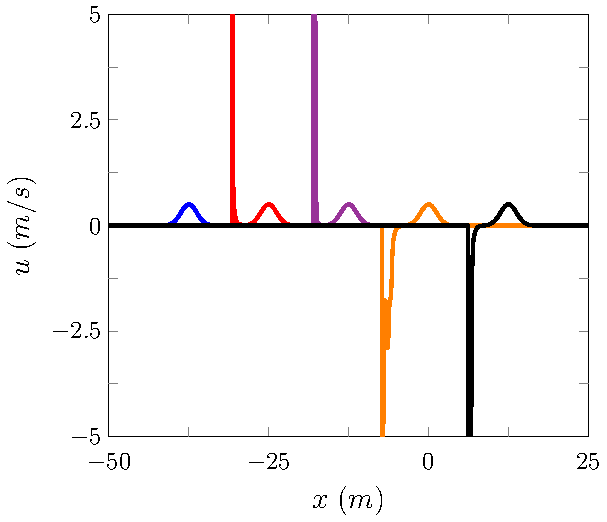
\includegraphics[width=\textwidth]{./chp5/figures/Forced/Dry/FDVMu.pdf}
		\subcaption{$u$}
	\end{subfigure}
	\caption{Plots of $w$, $b$, $h$, $G$ and $u$ produced by $\text{FDVM}_2$ with $\Delta x = 100 / 2^{10}m$ at $t=$ $0s$ ({\color{blue} \solidrule} / \squareF{blue} ), $2.5s$ ({\color{red} \solidrule}/ \squareF{red}), $5.0s$ ({\color{violet!80!white} \solidrule} / \squareF{violet!80!white}), $7.5s$ ({\color{orange} \solidrule}/ \squareF{orange}), $10.0s$ ({\color{black} \solidrule} / \squareF{black}) of the dry bed forced solution problem, where $a_0 = 0m$.}
	\label{fig:ForcedFDVMP2PExAll}
\end{figure}

These large errors in $u$ when $h$ is small are caused by the particular choices $h_{{base}} = 10^{-8}$ and $h_{{tol}}  = 10^{-12}$ used in the desingularisation transformation applied to the elliptic solver, \eqref{eqn:usolvefromGhb}. By choosing larger values of these quantities the errors in $u$ can be significantly damped. However, if $h_{{base}}$ and $h_{{tol}}$ are larger they dominate the $L_1$ errors for larger $\Delta x$ values making the convergence less obvious. This trade-off is present in all desingularisation transforms. 

For our purposes the chosen desingularisation transform \eqref{eqn:hdrytransform} with small $h_{{base}}$ and $h_{{tol}}$ values are sufficient, resulting in large observed errors in $u$ when $h$ is small.

The $L_1$ errors for $h$, $u$, $uh$ and $G$ for both methods are given in Figure \ref{fig:ForcedSolDryL1}. Both methods exhibit second-order convergence in all the quantities except $u$. This is because all the flux and source terms of the Serre equations \eqref{eqn:FullSerreCon} only depend on $u$ multiplied by some power of $h$; so that the large errors in $u$ when $h$ is small do not translate to significant errors in $G$, $h$ or $uh$. Indeed by restricting the $L_1$ errors to compare only the regions where $h > 10^{-3} m$ as in Figure \ref{fig:ForcedSolDryL1restrict}, we recover the expected second-order accuracy in all quantities.

Therefore, these methods can accurately handle the dry bed problem, even with small $h_{{base}}$ and $h_{{tol}}$ values, although in such cases the velocity may have large errors in regions where $h$ is small. 

\begin{figure}
	\centering
	\begin{subfigure}{0.5\textwidth}
		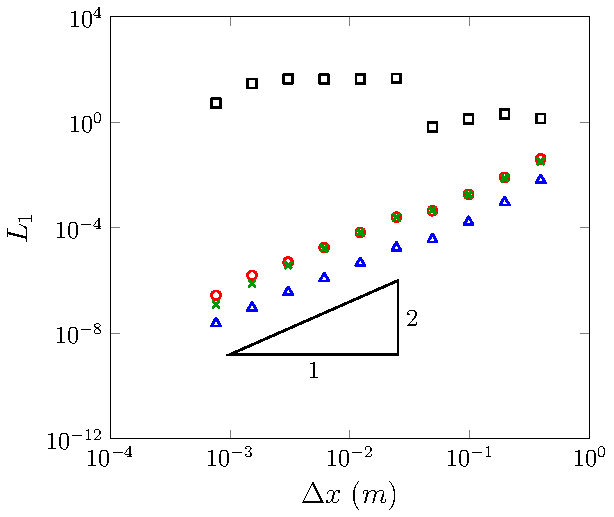
\includegraphics[width=\textwidth]{./chp5/figures/Forced/Dry/FEVML1.pdf}
		\subcaption{$\text{FEVM}_2$}
	\end{subfigure}%
	\begin{subfigure}{0.5\textwidth}
		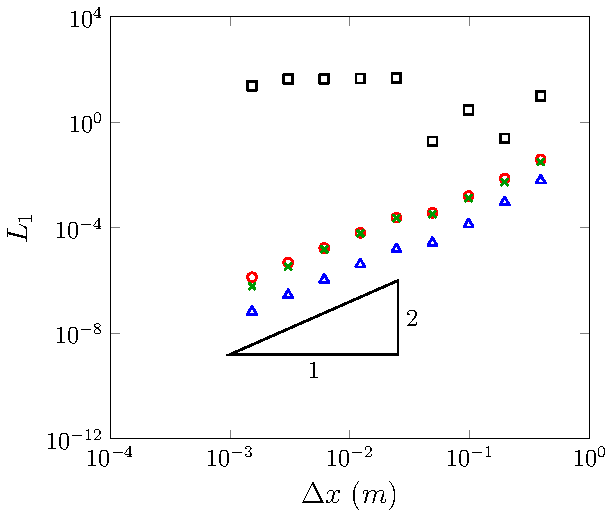
\includegraphics[width=\textwidth]{./chp5/figures/Forced/Dry/FDVML1.pdf}
		\subcaption{$\text{FDVM}_2$}
	\end{subfigure}
	\caption{Convergence plots as measured by the $L_1$ norm for $h$ (\trianglet{blue}), $u$ (\squaret{black}),  $uh$ ({\crosst{green!60!black}})  and $G$ (\circlet{red}) for the dry bed forced solution problem for FEVM and FDVM at $t=10s$.}
	\label{fig:ForcedSolDryL1}
\end{figure}

\begin{figure}
	\centering
	\begin{subfigure}{0.5\textwidth}
		\includegraphics[width=\textwidth]{./chp5/figures/Forced/Dry/FEVML1red.pdf}
		\subcaption{$\text{FEVM}_2$}
		\vspace{0.5cm}
	\end{subfigure}%
	%[]!!---!![]
	\begin{subfigure}{0.5\textwidth}
		\includegraphics[width=\textwidth]{./chp5/figures/Forced/Dry/FDVML1red.pdf}
		\subcaption{$\text{FDVM}_2$}
		\vspace{0.5cm}
	\end{subfigure}
	\caption{Convergence plots for regions where $h > 10^{-3}m$ as measured by the $L_1$ norm for $h$ (\trianglet{blue}), $u$ (\squaret{black}) and $G$ (\circlet{red}) for the dry bed forced solution problem for FEVM and FDVM at $t=10s$.}
	\label{fig:ForcedSolDryL1restrict}
\end{figure}

\medskip
In this chapter the analytic and forced solutions were used to assess the numerical methods. It was found that the hybrid finite volume methods performed better than the finite difference methods and that second-order methods were sufficient to accurately reproduce the analytic and forced solutions of the Serre equations.
